\section{Tổng quan về Data Warehouse}
\subsection{Khái niệm:}
Kho dữ liệu (Data Warehouse) được hiểu là một tập hợp các dữ liệu tương đối ổn định (không hay thay đổi), cập nhật theo thời gian, được tích hợp theo hướng chủ đề nhằm hỗ trợ quá trình tạo quyết định về mặt quản lý (W.H. Inmon).\\

Kho dữ liệu về bản chất là một cơ sở dữ liệu bình thường, các hệ quản trị cơ sở dữ liệu quản lý và lưu trữ nó như các cơ sở dữ liệu thông thường. Tuy nhiên, nó có thể quản lý dữ liệu lớn và hỗ trợ truy vấn. Nên điểm khác biệt giữa kho dữ liệu và cơ sở dữ liệu là ở quan niệm, cách nhìn nhận vấn đề.

\subsection{Đặc tính:}
\begin{enumerate}
    \item Hướng chủ đề: Cung cấp một khung nhìn đơn giản và súc tích xung quanh các sự kiện của các chủ đề ứng với mỗi loại tổ chức. Kho dữ liệu được thiết kế để hỗ trợ việc phân tích dữ liệu và hỗ trợ ra quyết định sau khi loại bỏ những dữ liệu không hữu ích.
    \item Tính tích hợp: Là đặc tính quan trọng nhất. Khi dữ liệu từ nhiều nguồn khác nhau đưa vào kho dữ liệu, chúng sẽ được chuyển đổi, định dạng lạ,.. để đảm bảo sự đồng nhất trong các quy ước tên, cấu trúc mã hóa, các đơn vị đo, thuộc tính,... giữa các nguồn khác nhau.
    \item Gắn thời gian và có tính lịch sử: Dữ liệu trong kho dữ liệu bao gồm cả quá khứ và hiện tại. Mỗi dữ liệu trong kho dữ liệu đều được gắn với thời gian và có tính lịch sử.
    \item Chỉ đọc, không biến động: Là một lưu trữ vật lý của dữ liệu được chuyển đổi từ môi trường tác nghiệp. Kho dữ liệu tách rời với môi trường tác nghiệp, nên dữ liệu trong đó là dữ liệu chỉ đọc, không chỉnh sửa hoặc thêm mới.
\end{enumerate}
\subsection{Lợi ích}
\begin{itemize}[label=$-$]
    \item Dữ liệu sau khi đưa vào kho dữ liệu đều tuần theo những quy tắc thống nhất.
    \item Dữ liệu được tổ chức tạo thuận lợi cho việc truy vấn phân tích và tạo tiền đề để đưa ra những quyết định có ảnh hưởng lớn.
    \item Cải thiện tính bảo mật và hiệu suất mà không cần tách động tới hệ thống dữ liệu gốc.
    \item Công việc kinh doanh trở nên thông minh hơn, nâng cao dịch vụ khách hàng.
\end{itemize}

\subsection{Kiến trúc:}
\subsubsection{Phân loại kiến trúc:}
Phụ thuộc rất nhiều vào vị trí của từng bộ phận trong tổ chức. Các kiến trúc phổ biến của kho dữ liệu bao gồm:
\begin{enumerate}
    \item \textbf{Kiến trúc cơ bản:}
    Kiến trúc cơ bản rất ít được sử dụng trong thực tế. Mặc dù, kiến trúc này loại bỏ dư thừa dữ liệu giúp giảm thiểu lượng dữ liệu được lưu trữ nhưng không phù hợp với các doanh nghiệp có yêu cầu dữ liệu phức tạp và nhiều nguồn dữ liệu. Trong kiến trúc cơ bản chỉ có tầng nguồn là tầng có sẵn về mặt vật lý. Kho dữ liệu của kiến trúc này là ảo tức nó được xây dựng dưới dạng một cái nhìn đa chiều về dữ liệu hoạt động và được tạo bởi phần mềm trung gian cụ thể hoặc một lớp xử lý trung gian.
    \begin{center}
            \begin{figure}[!h]
                \centering
                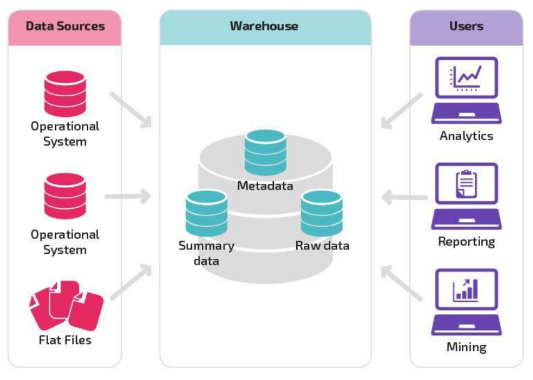
\includegraphics[scale = 1]{figures/Duyen/Kiến trúc kho dl cơ bản.PNG}
              \caption{Kiến trúc kho dl cơ bản}
            \end{figure}
\end{center}
    \item \textbf{Kiến trúc với vùng tập kết dữ liệu (Staging Area):} Kiến trúc này cung cấp thông tin luôn ở chất lượng tốt, ngay cả khi quyền truy cập vào các nguồn bị từ chối tạm thời vì lý do kỹ thuật hoặc tổ chức; truy vấn phân tích kho dữ liệu không ảnh hưởng đến việc quản lý các giao dịch, độ tin cậy cao, kho dữ liệu được cấu trúc logic theo mô hình đa chiều, kho dữ liệu có thể sử dụng các giải pháp thiết kế cụ thể để tối ưu hóa hiệu suất của các ứng dụng phân tích và báo cáo.
    \newpage
    \begin{center}
            \begin{figure}[!h]
                \centering
                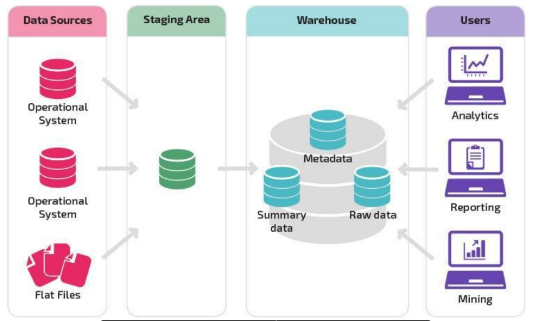
\includegraphics[scale = 1]{figures/Duyen/Kiến trúc kho dữ liệu vs Staging Area.PNG}
              \caption{Kiến trúc kho dữ liệu vs Staging Area}
            \end{figure}
\end{center}
    \item \textbf{Kiến trúc với vùng tập kết dữ liệu (Staging Area) và kho dữ liệu chủ đề (Data Marts):}
    Đây là kiến trúc phổ biến nhất trong ba loại. Ưu điểm chính của tầng tập kết dữ liệu (Staging Area) là tạo ra một mô hình dữ liệu tham chiếu chung cho cả doanh nghiệp. Đồng thời, tách biệt rõ ràng các vấn đề khai thác và tích hợp dữ liệu nguồn với các vấn đề của tổng thể kho dữ liệu. Đáng chú ý, tầng tập kết dữ liệu cũng được sử dụng trực tiếp để hoàn thành tốt một số nhiệm vụ hoạt động. Bên cạnh đó, kho dữ liệu chủ đề (Data Mart) giúp dữ liệu được truy cập dễ dàng hơn và cải thiện hiệu suất hệ thống.
     \begin{center}
            \begin{figure}[!h]
                \centering
                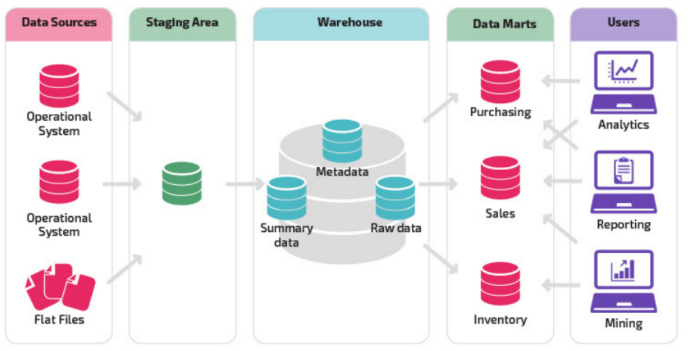
\includegraphics[scale = 1]{figures/Duyen/Kiến trúc kho dl với Staging và Data Marts.PNG}
              \caption{Kiến trúc kho dl với Staging và Data Marts}
            \end{figure}
    \end{center}
\end{enumerate}
    \subsubsection{Nguồn dữ liệu}
    Nguồn dữ liệu của kho dữ liệu rất đa dạng:
    \begin{itemize}[label=$-$]
        \item Dữ liệu từ các hệ thống tác nghiệp.
        \item Hệ thống kế thừa.
        \item Các nguồn dữ liệu bên ngoài.
    \end{itemize}
\subsubsection{Tập kết dữ liệu}
Tập kết dữ liệu (Data Staging) là nơi lưu trữ trung gian được sử dụng để xử lý dữ liệu trong thời gian chiết xuất, chuyển đổi và tải (ETL) quá trình. Dữ liệu tại đây có thể bị xóa trước khi chạy quy trình ETL hoặc ngay sau khi hoàn thành thành công quy trình ETL.\\
    Tuy nhiên, trong một số trường hợp Data Staging được thiết kế để
lưu giữ dữ liệu trong thời gian dài cho các mục đích lưu trữ hoặc xử lý sự cố.
\subsubsection{Công cụ trích xuất, chuyển đổi và tải dữ liệu}
Quy trình ETL được thiết kế phù hợp trích xuất dữ liệu từ hệ thống nguồn, thực thi các tiêu chuẩn về chất lượng và tính nhất quán của dữ liệu, tuân thủ dữ liệu để các nguồn riêng biệt có thể được sử dụng cùng nhau và cuối cùng cung cấp dữ liệu ở định dạng sẵn sàng trình bày để
các nhà phát triển ứng dụng có thể xây dựng ứng dụng và người dùng cuối có thể đưa ra quyết định.
\begin{enumerate}
    \item \textbf{Trích xuất (Extract):}
    Trích xuất dữ liệu một cách tạo tiền đề cho sự thành công của các
    quy trình tiếp theo. Hầu hết các dự án kho dữ liệu kết hợp dữ liệu từ các hệ thống nguồn khác nhau. Mỗi hệ thống riêng biệt cũng có thể sử dụng một tổ chức và/hoặc định dạng dữ liệu khác nhau. Việc truyền trực tuyến nguồn dữ liệu được trích xuất và tải nhanh chóng
    đến cơ sở dữ liệu đích là một cách khác để thực hiện ETL khi không cần lưu trữ dữ liệu trung gian. Quá trình trích xuất nhằm xác thực dữ liệu xem được lấy từ các nguồn có các giá trị chính xác hay không.
    \item \textbf{Biến đổi (Transform):}
    Trong giai đoạn chuyển đổi dữ liệu , một loạt các quy tắc hoặc chức năng được áp dụng cho dữ liệu được trích xuất để chuẩn bị cho việc tải vào mục tiêu cuối cùng. Một chức năng quan trọng của chuyển đổi là làm sạch dữ liệu, nhằm chuyển dữ liệu "thích hợp"đến mục tiêu. Việc tương tác giữa các hệ thống khác nhau gặp cản trở do các bộ ký tự có thể có sẵn trong hệ thống này nhưng có thể không có ở các hệ thống khác.
    \item \textbf{Load:}
    Tùy thuộc vào yêu cầu của tổ chức, quá trình tải dữ liệu rất khác nhau. Một số kho dữ liệu có thể ghi đè thông tin hiện có bằng thông tin tích lũy; cập nhật dữ liệu trích xuất thường xuyên được thực hiện theo chu kỳ. Các kho dữ liệu khác (hoặc thậm chí các phần khác của cùng một kho dữ liệu) có thể thêm dữ liệu mới ở dạng lịch sử theo các khoảng thời gian đều đặn. Thời gian và phạm vi thay thế hoặc kết nối thêm là các lựa chọn thiết kế chiến lược phụ thuộc vào thời gian có sẵn và nhu cầu của doanh nghiệp. Các hệ thống phức tạp hơn có thể duy trì lịch sử và dấu vết kiểm tra tất cả các thay đổi đối với dữ liệu được tải vào kho dữ liệu.\\
    Khi giai đoạn tải tương tác với cơ sở dữ liệu, các ràng buộc được xác định trong lược đồ cơ sở dữ liệu - cũng như trong các trình kích hoạt được kích hoạt khi tải dữ liệu - áp dụng. Ví dụ: Tính duy nhất, tính toàn vẹn tham chiếu, các trường bắt buộc), cũng góp phần vào hiệu suất chất lượng dữ liệu tổng thể của quy trình ETL.
\end{enumerate}
\subsubsection{Siêu dữ liệu}
Siêu dữ liệu (Metadata) lưu các định nghĩa logic các bảng, thuộc tính của kho dữ liệu, tên các nguồn dữ liệu tác nghiệp, định nghĩa vật lý các bảng và các cột.
\subsubsection{Kho dữ liệu chủ đề}
Kho dữ liệu chủ đề (Data Mart) có những đặc điểm giống với kho dữ liệu (Data Warehouse) nhưng với quy mô nhỏ hơn và lưu trữ dữ liệu về một lĩnh vực, một chuyên ngành. Các kho dữ liệu chủ đề có thể được hình thành từ một tập con dữ liệu của kho dữ liệu hoặc cũng có thể được
xây dựng độc lập và sau khi xây dựng xong, các kho dữ liệu chủ đề có thể được kết nối tích hợp lại với nhau tạo thành kho dữ liệu. Vì vậy có thể xây dựng kho dữ liệu bắt đầu bằng việc xây dựng các kho dữ liệu chủ đề hay ngược lại xây dựng kho dữ liệu trước sau đó tạo ra các kho dữ
liệu chủ đề.
\subsubsection{Các công cụ và nền tảng hỗ trợ}
\begin{itemize}[label=$-$]
    \item Hệ quản trị CSDL: MySQL, Oracle, Microsoft SQL Server, MariaDB,..
    \item Trực quan hoá dữ liệu, tạo báo cáo (Report, Dashboard): Power BI, Tableau,...
    \item Phân tích dữ liệu: Python, R, SAS, Excel. Orange...
\end{itemize}
\subsection{Kiến trúc khối và Các dạng lược đồ dữ liệu đa chiều}
\subsubsection{Mô hình dữ liệu đa chiều}
Data Warehouse và các hệ thông OLAP được xây dựng theo mô hình dữ liệu đa chiều. Dữ liệu trong kho dữ liệu được thể hiện dưới dạng đa chiều gọi là khối (Cube). Mỗi chiều mô tả một đặc trưng nào đó của dữ liệu. (Nếu số chiều dữ liệu lớn hơn 3, gọi là Hyper Cube).
\begin{enumerate}
    \item \textbf{Chiều (Dimension) \& Độ đo (Measure)}
    \begin{itemize}[label=$-$]
        \item Chiều cung cấp các thông tin, ngữ cảnh của bảng Fact.
        \item Độ đo là đại lượng có thể tính toán được trên các thuộc tính của bảng Fact.
    \end{itemize}
    \item \textbf{Cây phân cấp \& Số liệu tổng hợp}
    \begin{itemize}[label=$-$]
        \item Mức độ chi tiết của các tiêu chí thể hiện cho người dùng được gọi là mức dữ liệu, được quyết định bằng việc kết hợp các mức dữ liệu của từng phân lớp.
        \item Số liệu tổng hợp: Việc tổng hợp số liệu xảy ra khi người dùng thay đổi mức chi tiết của dữ liệu lấy ra từ Cube, bằng cách duyệt qua cây phân cấp.
    \end{itemize}
    \item  \textbf{Các mô hình thiết kế Date Warehouse}
    \begin{itemize}[label=$-$]
        \item OLAP kiểu quan hệ (Relational OLAP $\sim$ ROLAP)
        \item OLAP kiểu đa chiều (Multi-dimensional OLAP $\sim$ MOLAP)
        \item OLAP kết hợp (Hybird OLAP HOLAP = ROLAP + MOLAP)
    \end{itemize}
    \begin{center}
            \begin{figure}[!h]
                \centering
                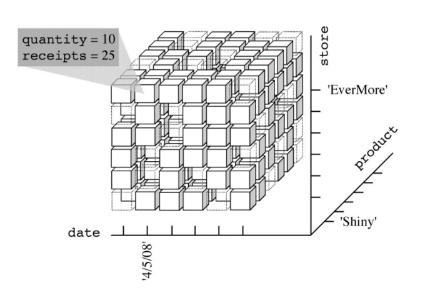
\includegraphics[scale = 1]{figures/Duyen/Minh họa khối dữ liệu.PNG}
              \caption{Minh họa khối dữ liệu}
            \end{figure}
\end{center}
\end{enumerate}
\subsubsection{Lược đồ dữ liệu đa chiều}
\begin{enumerate}
\item \textbf{Lược đồ hình sao}\\
Gồm 1 bảng Fact nằm ở trung tâm và những bảng Dimension bao quanh. Các câu hỏi nhằm vào bảng Fact và được cấu trúc bởi các bảng Dimension.
\begin{itemize}
    \item  Ưu điểm: Bảng Fact, Dimension được mô tả rõ ràng, dễ hiểu. Bảng Dim chứa dữ liệu tĩnh, và bảng Fact chứa dữ liệu động được nạp bằng các thao tác. Khoá của Fact được tạo bởi khoá của các bảng Dim. Nghĩa là khoá chính của các bảng Dim chính là khoá ngoại của bảng Fact.
    \item Nhược điểm: Dữ liệu không được chuẩn hoá
\end{itemize}
\item \textbf{Lược đồ hình bông tuyết}\\
Lược đồ hình bông tuyết là một sự mở rộng của lược đồ hình sao tại đó mỗi "cánh ngôi sao". Các chiều được cấu trúc rõ ràng. Bảng Dimension được chia thành hai chiều: chính và phụ.
\begin{itemize}
    \item Ưu điểm: Số chiều được phân cấp thể hiện dạng chuẩn của bảng Dimension.
    \item Nhược điểm: Cấu trúc phi dạng chuẩn của lược đồ hình sao phù hợp hơn cho việc duyệt các chiều.
\end{itemize}
\item \textbf{Lược đồ ngân hà}\\
Lược đồ ngân hà được hình thành nhờ sự kết hợp giữa lược đồ hình sao và lược đồ hình bông tuyết. Lược đồ này chứa nhiều bảng Fact sử dụng chung một số bảng Dim và là sự kết hợp của nhiều Data Mart.
\end{enumerate}